\documentclass[14pt]{beamer} 
% \usepackage[utf8]{inputenc}
% \usepackage{xeCJK}
\usepackage{graphicx}
\usepackage {mathtools}
\usepackage{newtxtext,newtxmath}
% \usepackage{utopia} %font utopia imported
\usetheme{CambridgeUS}
\usecolortheme{dolphin}

% set colors
\definecolor{myNewColorA}{RGB}{34,139,34}
\definecolor{myNewcolorA}{RGB}{34,139,34}
\definecolor{myNewcolorA}{RGB}{34,139,34}
\setbeamercolor{block title}{bg=myNewColorA,fg=black}
\setbeamercolor{block body}{bg=myNewColorA!20,fg=black}
\setbeamercolor{block title alerted}{bg=black, fg=myNewColorA}
\setbeamercolor{block body alerted}{bg=black!20, fg=black}

\setbeamercolor*{block title example}{bg=myNewColorA, fg = black}
\setbeamercolor*{block body example}{bg=myNewColorA!20, fg = black}
\usebeamercolor[myNewColorA]{block title alerted}
\setbeamercolor*{palette primary}{bg=myNewcolorA}
\setbeamercolor*{palette secondary}{bg=myNewcolorA, fg = white}
\setbeamercolor*{palette tertiary}{bg=myNewColorA, fg = white}
\setbeamercolor*{titlelike}{fg=myNewColorA}
\setbeamercolor*{title}{bg=myNewColorA}
\setbeamercolor*{item}{fg=myNewColorA}
\setbeamercolor*{caption name}{fg=myNewColorA}
\usefonttheme{professionalfonts}
\usepackage{hyperref}
%------------------------------------------------------------
% \titlegraphic{\includegraphics[height=1.5cm]{photo.png}} 

\setbeamerfont{title}{size=\large}
\setbeamerfont{subtitle}{size=\small}
\setbeamerfont{author}{size=\small}
\setbeamerfont{date}{size=\small}
\setbeamerfont{institute}{size=\small}
\setbeamerfont{collaborators}{size=\small}
\title[]{Image Classification by Reinforcement Learning With Two-State Q-Learning}


\author{ECSE 626 Final Project by Evelyn Hubbard}
\institute[]{Original Paper by: Abdul Mueed Hafiz [1]}
\date[\textcolor{white}{\today} ]
{\today}

%------------------------------------------------------------
%This block of commands puts the table of contents at the 
%beginning of each section and highlights the current section:
%\AtBeginSection[]
%{
%  \begin{frame}
%    \frametitle{Contents}
%    \tableofcontents[currentsection]
%  \end{frame}
%}
\AtBeginSection[]{
  \begin{frame}
  \vfill
  \centering
  \begin{beamercolorbox}[sep=8pt,center,shadow=true,rounded=true]{title}
    \usebeamerfont{title}\insertsectionhead\par%
  \end{beamercolorbox}
  \vfill
  \end{frame}
}
%------------------------------------------------------------
\begin{document}
%The next statement creates the title page.
\frame{\titlepage}
% \begin{frame}
% \frametitle{Table of Contents}
% \tableofcontents
% \end{frame}

%------------------------------------------------------------
    \begin{frame}{Introduction}
    \frametitle{Presentation Outline}
        \begin{enumerate}
            \item Paper Introduction and Context
            \item Image Classification and Active Learning Background
            \item Model Architecture
            \item Reinforcement Learning Background
            \item Hafiz's Two-State Q-Learning Algorithm
            \item Original Paper Results
            \item ECSE 626 Project Contributions and Results
            \item Paper Critiques and Suggestions
        \end{enumerate}
    \end{frame}
%------------------------------------------------------------
\begin{frame}{Introduction}
    \fontsize{12pt}{7.2}\selectfont
\begin{itemize}
    \item Image classification: traditionally solved by supervised learning techniques.
    \item Reinforcement learning (RL): method for learning optimal policies in sequential decision-making problems.
    \item Active vision: acquires multiple observati
    ons and \textbf{selects} parameters of the observation process
    \end{itemize}
    \begin{figure}
        \centering
        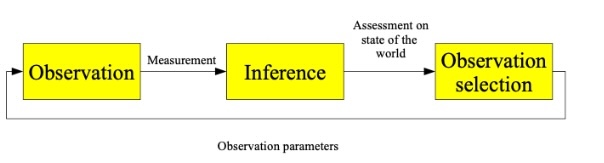
\includegraphics[width=0.75\textwidth]{activeloop.jpg}
        \caption{Active Vision Loop, adapted from [2]}
    \end{figure}
\end{frame}
%------------------------------------------------------------
\begin{frame}{Hafiz's 2022 Paper Context}
    \fontsize{12pt}{7.2}\selectfont
\begin{itemize}
    \item Deep Q-networks integrated RL with deep learning and demonstrated Q-learning's applicability to high-dimensional data [3]
    \item Connection with computer vision was prevalent from around 2015 to 2020 (ex: landmark detection) [3]
    \item Motivation for Hafiz's paper [1]:
    \begin{itemize}
        \item Image resolution selection 
        \item Reconstruction of digits using feature maps
        \item Earlier RL and image classification work with the goal of learning effective transformations on images (pre-classification)
    \end{itemize}
\end{itemize}
\end{frame}
%------------------------------------------------------------
\begin{frame}{Novelty of Hafiz's Paper}
    \textbf{Hafiz's paper proposed two new ideas [1]:}
    \begin{enumerate}
        \item New action: rotation
        \item Two-state Q-learning algorithm: instead of using the image as the state, the state is "better" or "worse" depending on the standard deviation of classification predictions after an action is taken 
    \end{enumerate}

\end{frame}
%------------------------------------------------------------
\begin{frame}{Model Architecture}
    \textbf{Three model components:}
    \begin{enumerate}
        \item Feature extracting CNN (predicts a class for a given image)
        \item Classifying structure (predicts a class for a feature map)
        \item Reinforcement learning algorithm (two-state Q-Learning on feature-maps to improve classification)
    \end{enumerate}
\end{frame}
%------------------------------------------------------------
\begin{frame}{Deep Learning:}
\fontsize{14pt}{7.2}\selectfont
    \begin{columns}
        % Column for the text
        \begin{column}{0.5\textwidth}
            \begin{itemize}
                \item The CNN is composed of a pre-trained base (ResNet50 ImageNet) and custom fine-tuned layers.
                \item The secondary classifier (an NN or SVM) is trained on the feature maps for a training set of images.
            \end{itemize}
        \end{column}
        % Column for the image
        \begin{column}{0.5\textwidth}
            \centering
            \begin{figure}
                \centering
                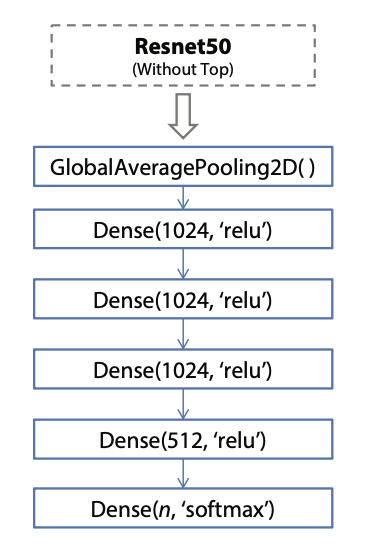
\includegraphics[width=0.60\textwidth]{NNarchitecture.png}
                \caption{Custom NN layers added to ResNet50 from [1]}
            \end{figure}
            %\captionof{figure}{NN for classification, adapted from [1]}
        \end{column}
    \end{columns}
\end{frame}
%------------------------------------------------------------
\begin{frame}{Model Architecture}
    \begin{figure}
        \centering
        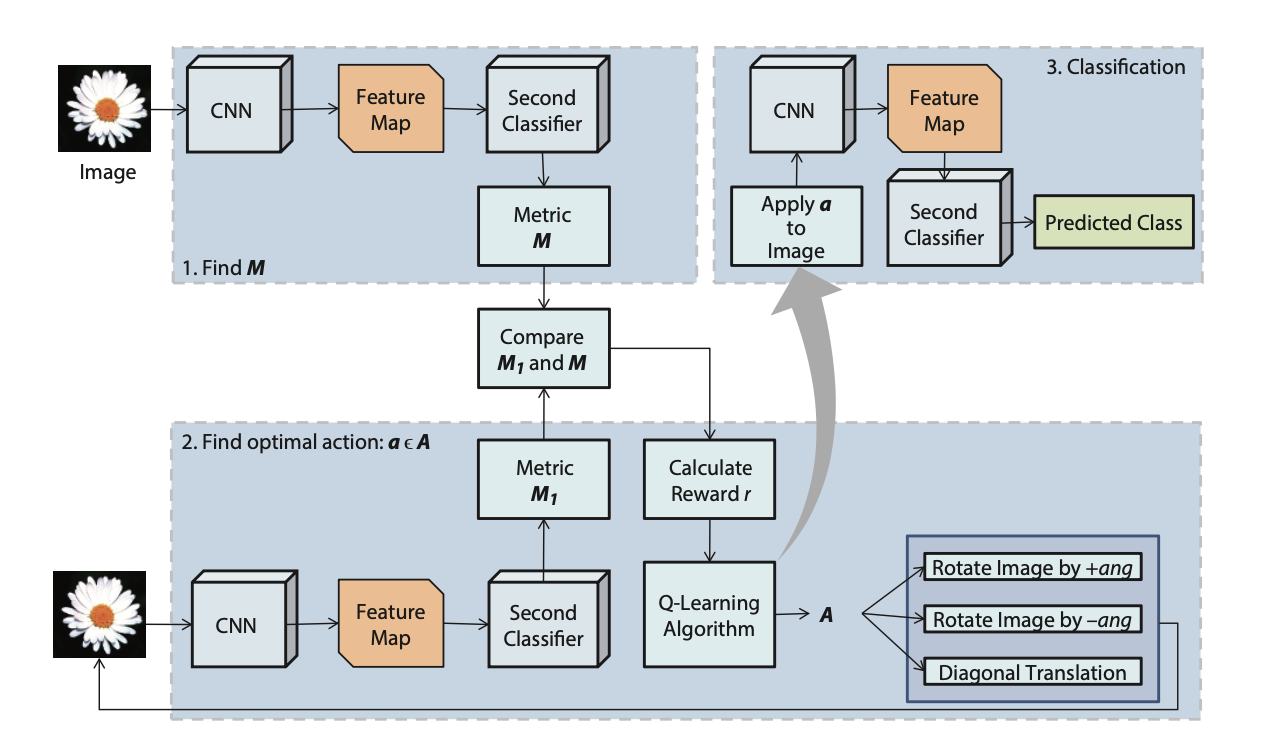
\includegraphics[width=0.85\textwidth]{model.png}
        \caption{Model Architecture[1]}
    \end{figure}
\end{frame}
%------------------------------------------------------------
%------------------------------------------------------------
\begin{frame}{Reinforcement Learning}
\end{frame}

\begin{frame}{Reinforcement Learning}
\begin{itemize}
    \item Markov Chain and trainsition kernel....
    \item reward function
    \item Reinforcement learning is a type of machine learning that involves an agent learning to make decisions by interacting with an environment.
    \item The agent receives rewards or penalties based on its actions, and its goal is to learn a policy that maximizes its cumulative reward.
    \item Q-learning is a popular reinforcement learning algorithm that learns a Q-function, which estimates the expected reward of taking an action in a given state.
    \item The Q-function is used to determine the best action to take in a given state.
\end{itemize}
\end{frame}
%------------------------------------------------------------
\begin{frame}{Structural Results of Reinforcement Learning}
\end{frame}
%------------------------------------------------------------
\begin{frame}{Two-State Q-Learning}
\begin{itemize}
    \item The two-state Q-learning algorithm uses a predictor to approximate the state of the environment.
    \item The predictor is trained to predict the next state of the environment given the current state and action.
    \item The Q-function is then learned using the predicted state instead of the true state.
    \item This reduces the state-action space and allows the agent to learn a policy more efficiently.
\end{itemize}
\end{frame}
%------------------------------------------------------------
\begin{frame}{Connection to Model}
\end{frame}
%------------------------------------------------------------
\begin{frame}{Paper's Results}
\end{frame}
%------------------------------------------------------------
\begin{frame}{My Contributions and Results}
\end{frame}
%------------------------------------------------------------
\begin{frame}{Paper Critiques}
\end{frame}
%------------------------------------------------------------
\begin{frame}{Suggestions}
\end{frame}
%------------------------------------------------------------
\begin{frame}{Discussion}
\end{frame}
%------------------------------------------------------------
\begin{frame}{Conclusion}
\textbf{Comparing the approximation schemes:}
    \begin{itemize}
        \item Sliding window method: computationally efficient, insensitive to initialization, requires a strong form of filter stability
        
        \item Quantized state space method: works under weaker stability conditions, sensitive to initialization, computationally more complex\newline\newline
    \end{itemize}
\textbf{Future research} could extend these methods to scenarios with noisy channels, channels with feedback, or systems with infinite state/action spaces.
\end{frame}
\begin{frame}{References:}
\fontsize{8pt}{7.2}\selectfont
[1]	A. M. Hafiz, “Image Classification by Reinforcement Learning With Two-State Q-Learning,” in Handbook of Intelligent Computing and Optimization for Sustainable Development, John Wiley and Sons, Ltd, 2022, pp. 171-181. doi: 10.1002/9781119792642.ch9.\newline
[2] C. Laporte, "Active Vision for Doctors in the Making," presented in *ECSE-626: Statistical Computer Vision*, Fall 2024, McGill University, Montreal, QC, Canada.\newline
[3]	N. Le, V. S. Rathour, K. Yamazaki, K. Luu, and M. Savvides, “Deep reinforcement learning in computer vision: a comprehensive survey,” Artif Intell Rev, vol. 55, no. 4, pp. 2733–2819, Apr. 2022, doi: 10.1007/s10462-021-10061-9.

    % \bibliographystyle{IEEEtran}
    % \bibliography{ECSE 626}
\end{frame}

\section*{Acknowledgement}  
\begin{frame}
\textcolor{myNewColorA}{\Huge{\centerline{Thank you!}}}
\end{frame}

\end{document}



